\section{Pruebas de funcionalidad}
La implementación del \textit{Backend} concluyó con pruebas de funcionalidad a cada uno de los
\textit{endpoints} que la API ofrece, con el fin de garantizar que cada uno de ellos realiza correctamente
las operaciones esperadas.
La colección de Postman ofrece una prueba de éxito para cada uno de los \textit{endpoints}, al ser
un entorno de pruebas iterativo, se pueden modificar \textit{queries} de los \textit{endpoints} o bien
los \textit{body} de las peticiones para comprobar manejo de errores, validación y autorización.

La prueba de funcionalidad para cada verbo HTTP se considera exitosa si la respuesta cumple con lo siguiente:
\begin{itemize}
    \item \textbf{GET}: El resultado contiene el código HTTP 200, un mensaje de éxito indicando que se obtuvieron
        los recursos y la información solicitada correctamente filtrada por los parámetros de la consulta,
        si es que se incluyen, en la sección de \textit{data}.
    \item \textbf{POST}: El resultado contiene el código HTTP 201, un mensaje de éxito indicando que el
        recurso se creó correctamente y un objeto \textit{data} con información importante del nuevo recurso.
        Además, el recurso debe estar creado en la base de datos con la información correspondiente y que exista en el Bucket S3, si aplica.
    \item \textbf{PUT}: El resultado contiene el código HTTP 200, un mensaje de éxito indicando que el recurso
        se actualizó correctamente y un objeto \textit{data} con información importante del recurso actualizado.
        Además, el recurso debe de estar actualizado en la base de datos con la información correspondiente.
    \item \textbf{PATCH}: El resultado contiene el código HTTP 200, un mensaje de éxito indicando que el recurso
        se actualizó correctamente y un objeto \textit{data} con información importante del recurso actualizado.
        Además, el recurso debe de estar actualizado en la base de datos con la información correspondiente.
    \item \textbf{DELETE}: El resultado contiene el código HTTP 200, un mensaje de éxito indicando que el recurso
        se eliminó correctamente. Además, el recurso eliminado se espera que ya no exista en la base de datos
        y que se elimine del Bucket S3, si aplica.
\end{itemize}

A continuación, se mostrarán resultados obtenidos para algunos de los \textit{endpoints} de la API, la lista completa de pruebas se encuentra en
el Anexo \ref{anexo:listaendpoints}.
\begin{itemize}
    \item \texttt{POST /auth/register}: Esta solicitud permite registrar a un nuevo usuario en la plataforma.
        Dentro del \textit{body} se incluyen los datos requeridos para cada tipo de usuario. El resultado esperado
        para esta prueba es un código de respuesta HTTP 201 con un mensaje de éxito y \textit{data} importante del
        nuevo usuario. Además, se espera que el usuario reciba un correo electrónico de verificación. 
            \begin{figure}[H]
                \centering
                \begin{minipage}{0.44\textwidth}
                    \centering
                    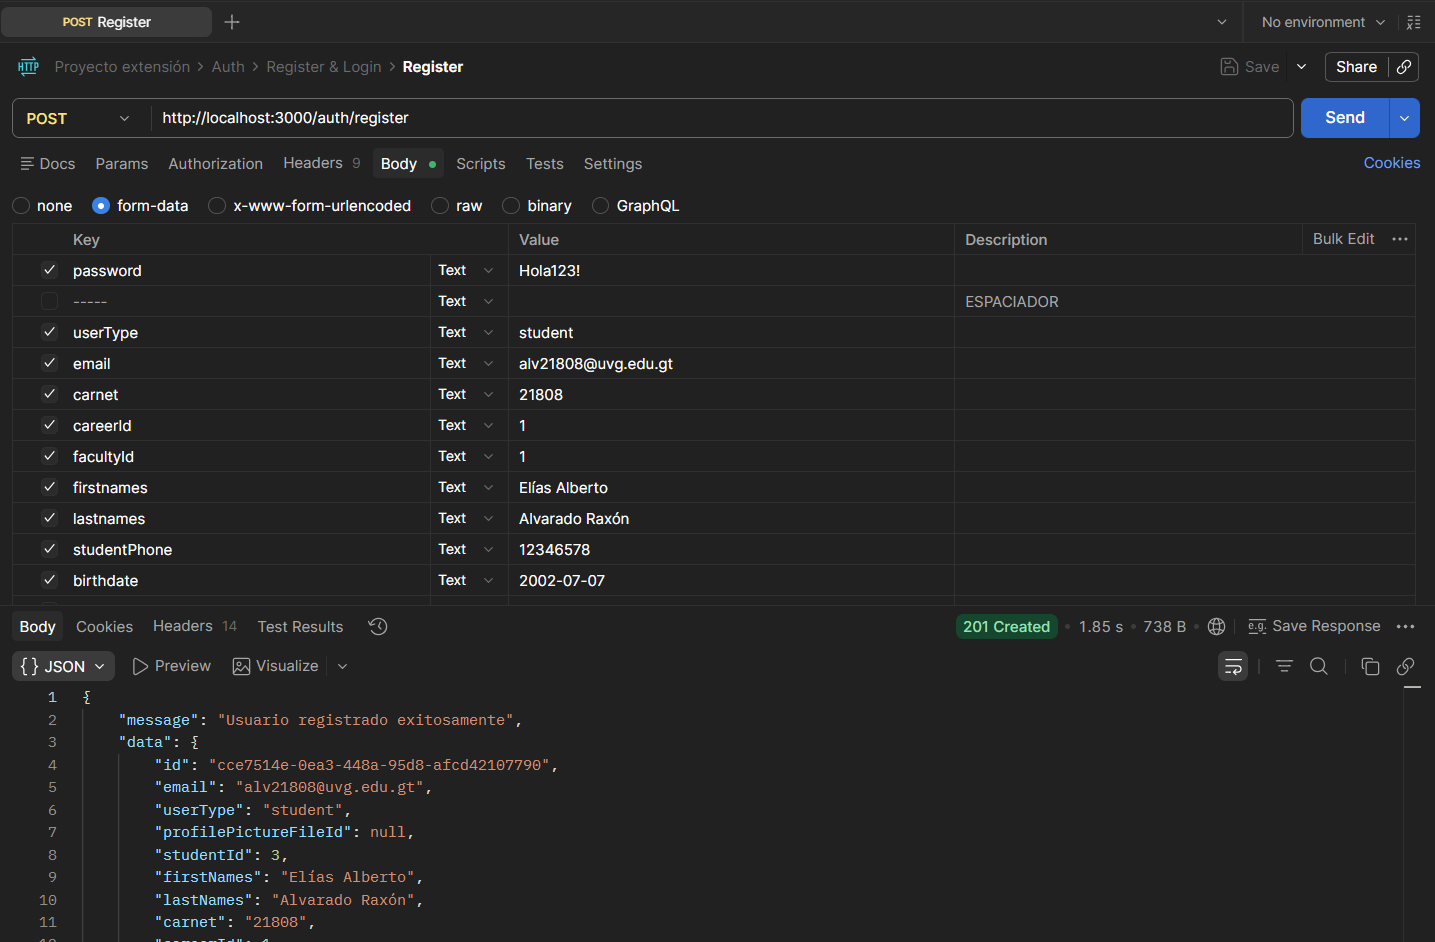
\includegraphics[width=\textwidth]{assets/studentRegister.png}
                    \subcaption{Registro de Estudiante - Prueba de éxito}
                \end{minipage}
                \begin{minipage}{0.44\textwidth}
                    \centering
                    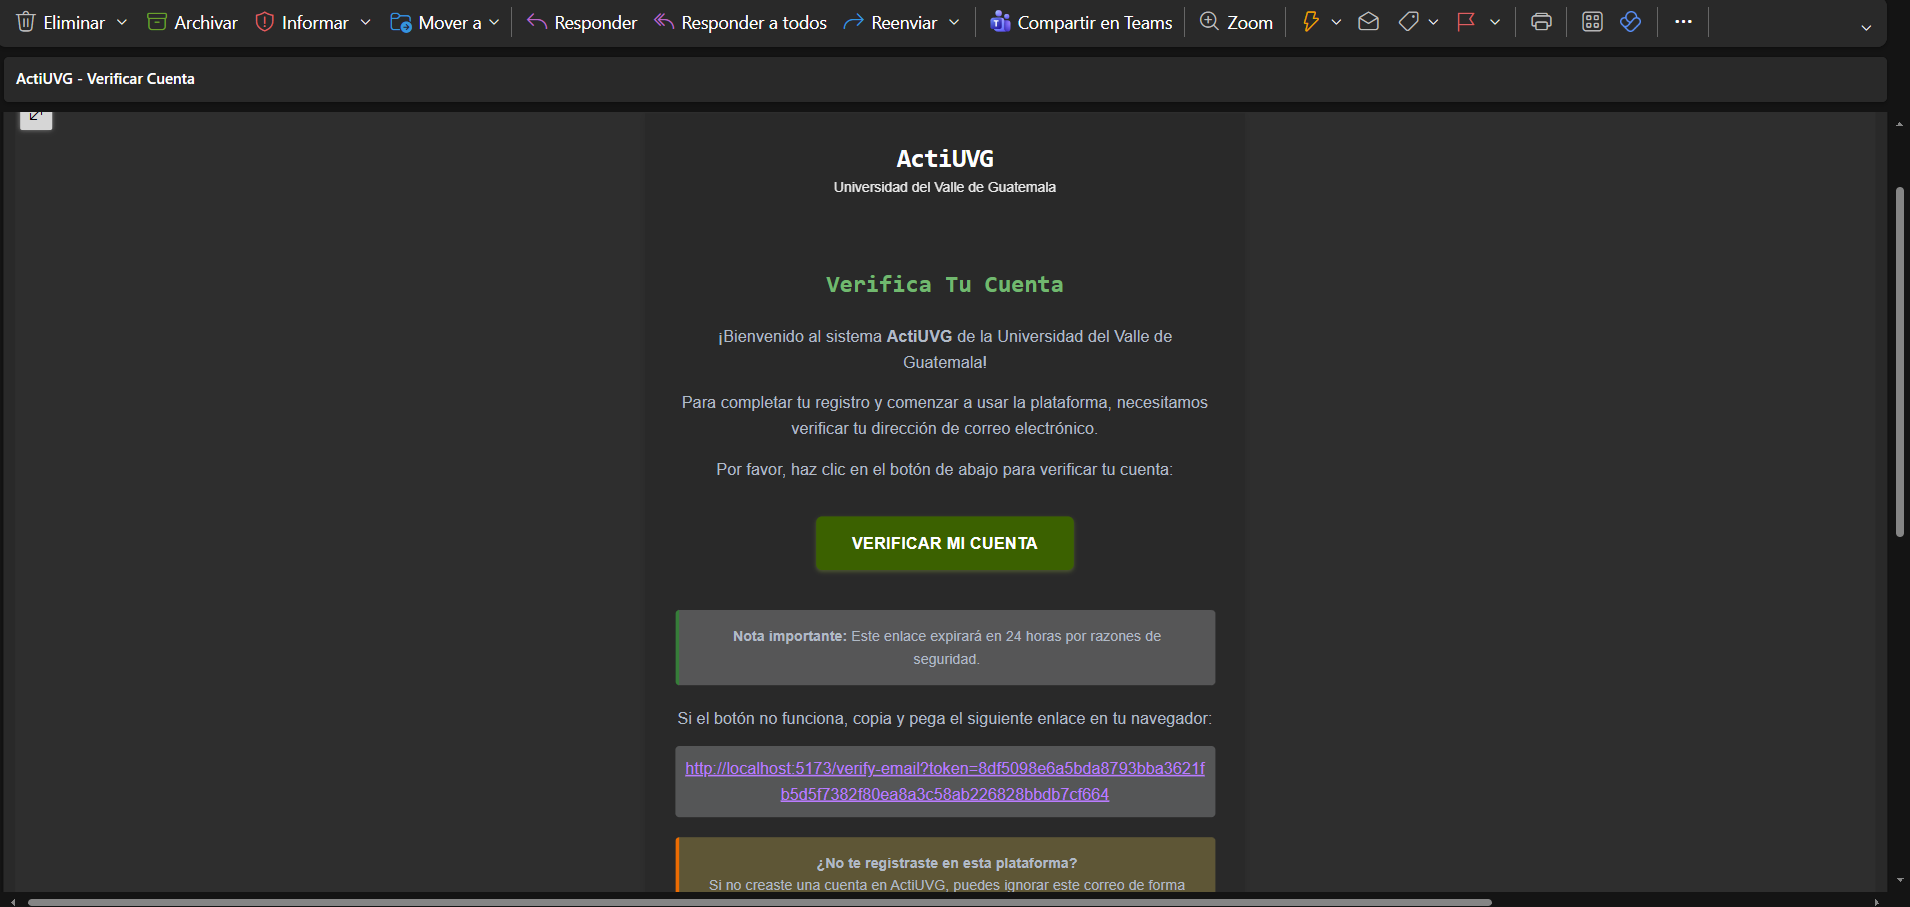
\includegraphics[width=\textwidth]{assets/verifyEmail.png}
                    \subcaption{Correo electrónico para verificación}
                \end{minipage}
                \caption{Registro de usuario y correo de verificación}
                \label{fig:studentRegister}
            \end{figure}
        Al intentar registrar a un usuario sin alguno de los campos requeridos, se espera que el resultado sea un
        código de respuesta HTTP 400 con un mensaje de error indicando que faltan campos requeridos.
            \begin{figure}[H]
                \centering
                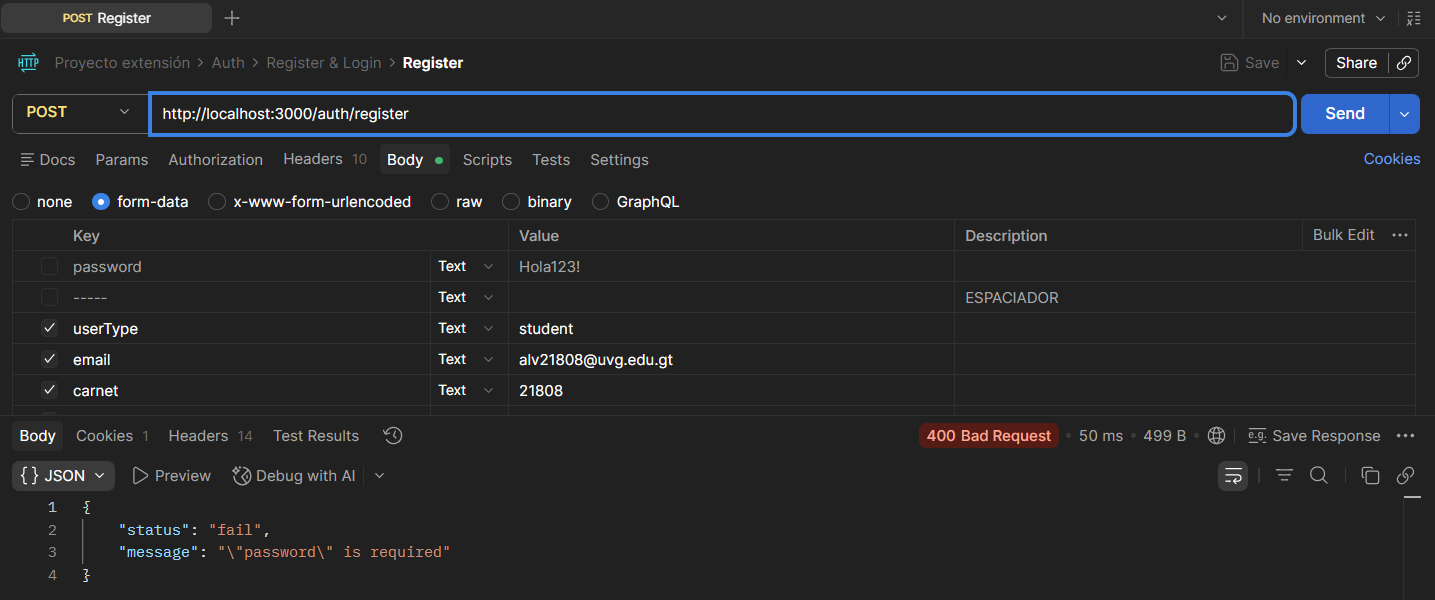
\includegraphics[width=0.88\textwidth]{assets/registerBadRequest.png}
                \caption{Registro de usuario con campos faltantes - Prueba de error}
                \label{fig:registerBadRequest}
            \end{figure}
    \item \texttt{GET /projects}: Esta solicitud permite obtener una lista de proyectos disponibles en la plataforma. El resultado esperado
        para esta prueba es un código de respuesta HTTP 200 con el listado de proyectos en la sección de \textit{data}.
            \begin{figure}[H]
                \centering
                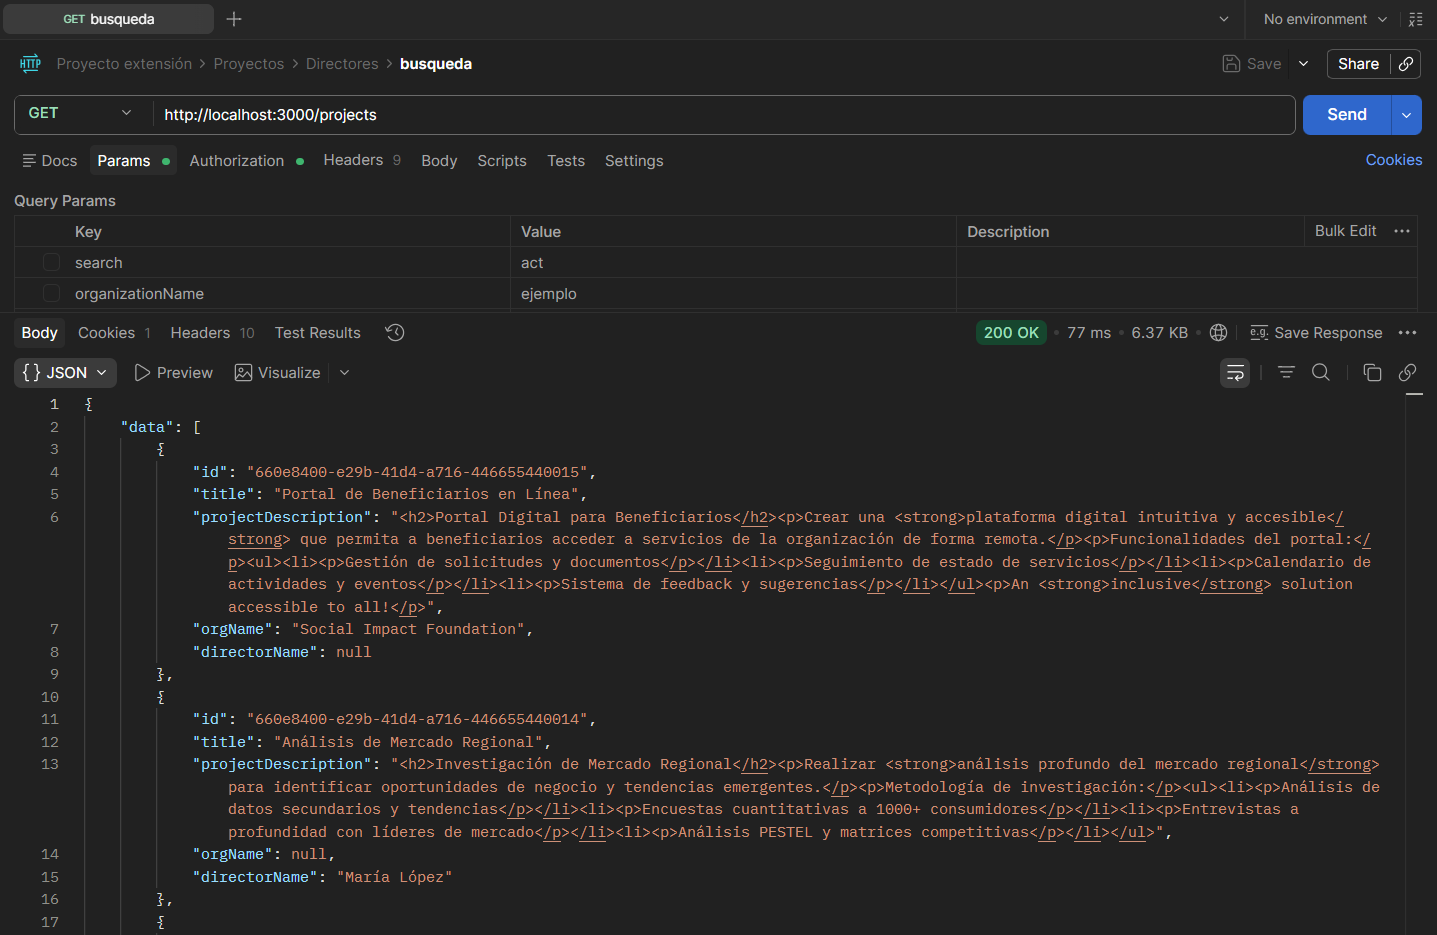
\includegraphics[width=0.88\textwidth]{assets/getProjects.png}
                \caption{Obtención de proyectos - Prueba de éxito}
                \label{fig:getProjects}
            \end{figure}
        Al no incluir un token de autenticación en la solicitud, se espera que el resultado sea un código de respuesta HTTP 401 con un
        mensaje de error indicando que el acceso fue denegado.
            \begin{figure}[H]
                \centering
                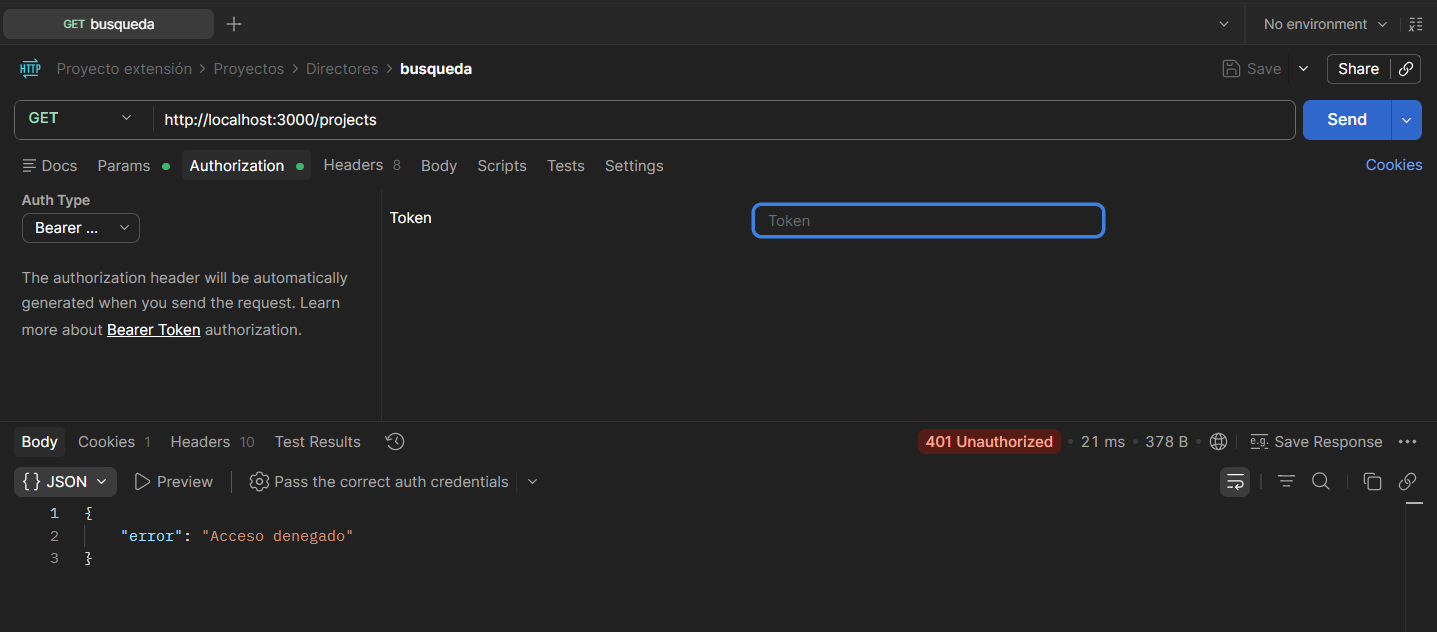
\includegraphics[width=0.88\textwidth]{assets/getProjectsUnauthorized.png}
                \caption{Obtención de proyectos sin autenticación - Prueba de error}
                \label{fig:getProjectsUnauthorized}
            \end{figure}
    \item \texttt{PUT /projects/:projectId}: Esta solicitud permite actualizar la información de un proyecto. El resultado esperado
        para esta prueba es un código de respuesta HTTP 200 con un mensaje de éxito y la información actualizada del proyecto en la sección de \textit{data}.
        En caso que un usuario que no es el creador del proyecto intente actualizarlo, se espera que el resultado sea un código de respuesta HTTP 403 con un
        mensaje de error indicando que no tiene permisos para realizar la acción.
            \begin{figure}[H]
                \centering
                \begin{minipage}{0.44\textwidth}
                    \centering
                    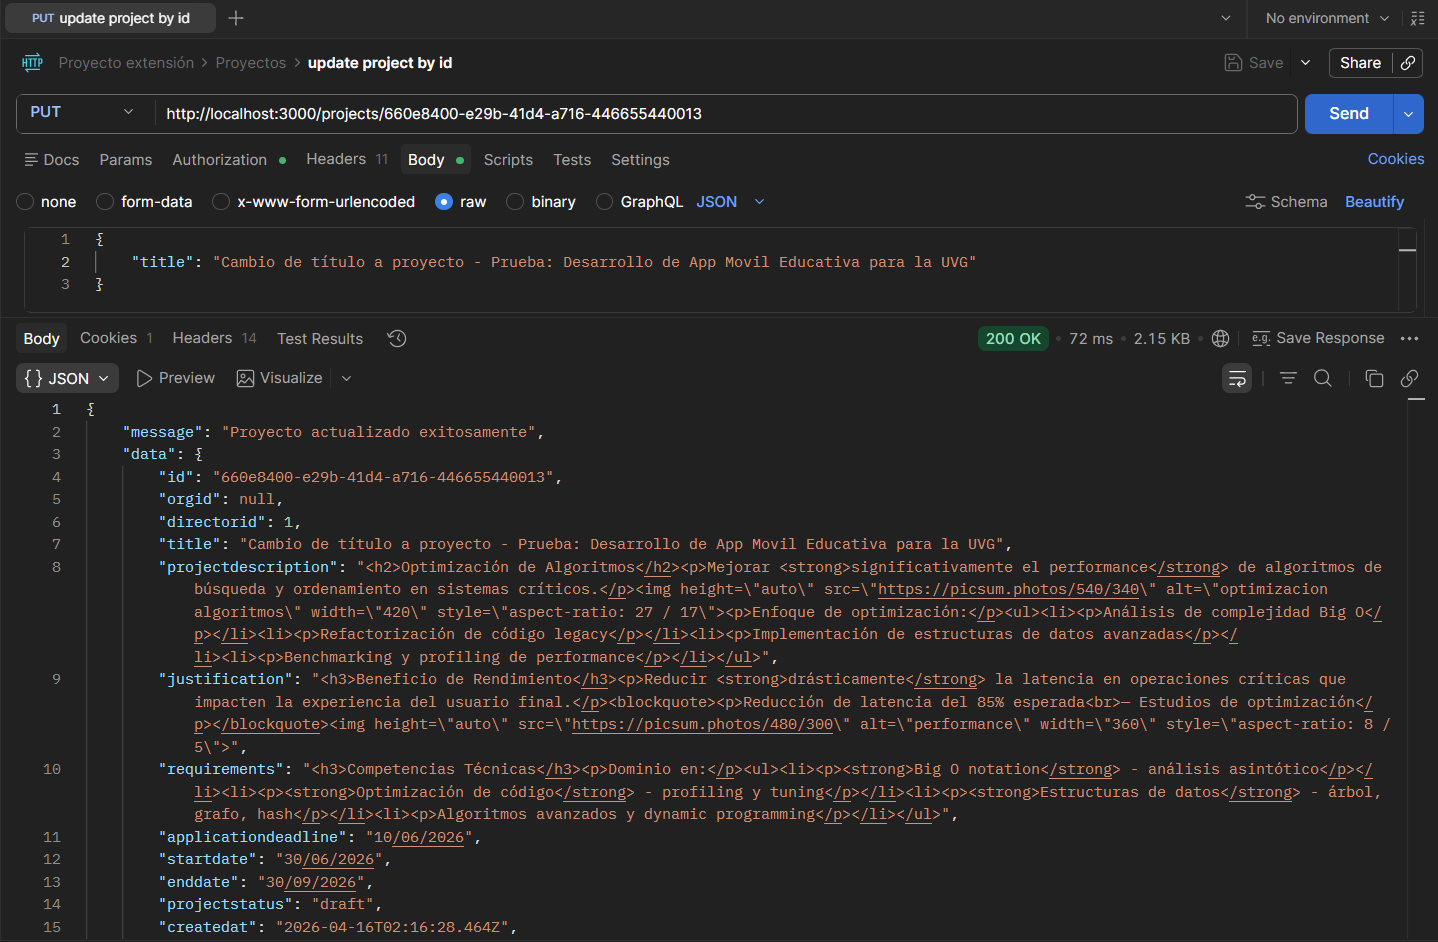
\includegraphics[width=0.88\textwidth]{assets/updateProject.png}
                    \subcaption{Actualización de proyecto - Prueba de éxito}
                \end{minipage}
                \begin{minipage}{0.44\textwidth}
                    \centering
                    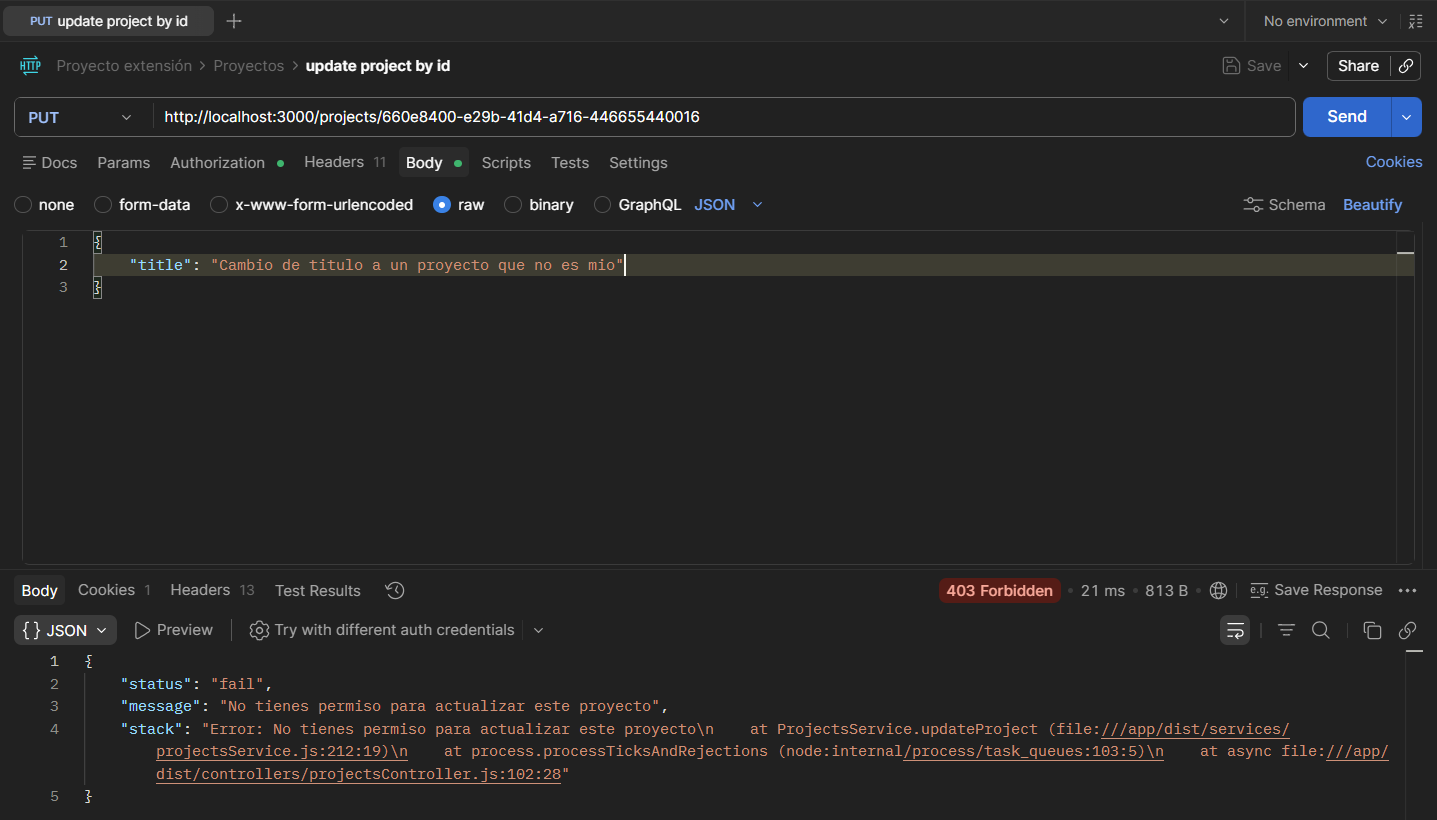
\includegraphics[width=\textwidth]{assets/updateProjectUnauthorized.png}
                    \subcaption{Actualización de proyecto por usuario no autorizado - Prueba de error}
                \end{minipage}
                \caption{Actualización de proyecto}
                \label{fig:updateProject}
            \end{figure}
    \item \texttt{PATCH /projects/:projectId/status}: Esta solicitud permite actualizar el estado de un proyecto. El resultado esperado
        para esta prueba es un código de respuesta HTTP 200 con un mensaje de éxito y la información actualizada del proyecto en la sección de \textit{data}.
            \begin{figure}[H]
                \centering
                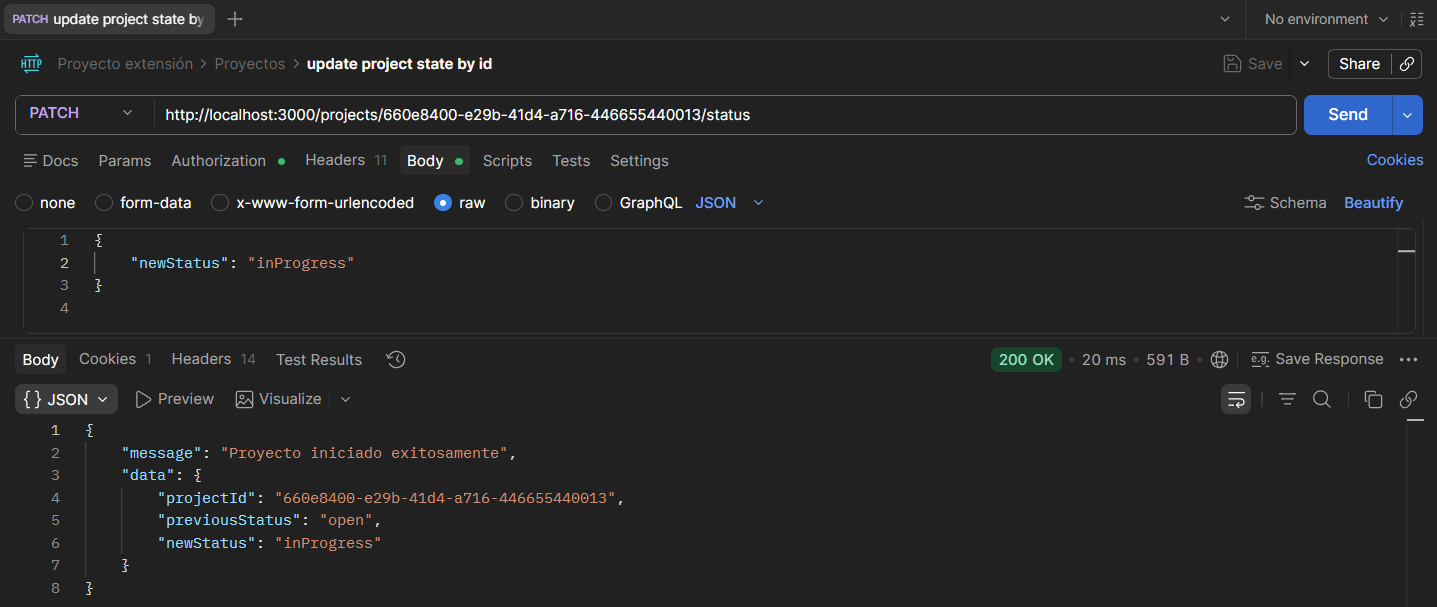
\includegraphics[width=0.88\textwidth]{assets/updateProjectStatus.png}
                \caption{Actualización de estado de proyecto - Prueba de éxito}
                \label{fig:updateProjectStatus}
            \end{figure}
    \item \texttt{DELETE /projects/:projectId/resources/:fileId}: Esta solicitud permite eliminar un recurso asociado a un proyecto. El resultado esperado
        para esta prueba es un código de respuesta HTTP 200 con un mensaje de éxito.
            \begin{figure}[H]
                \centering
                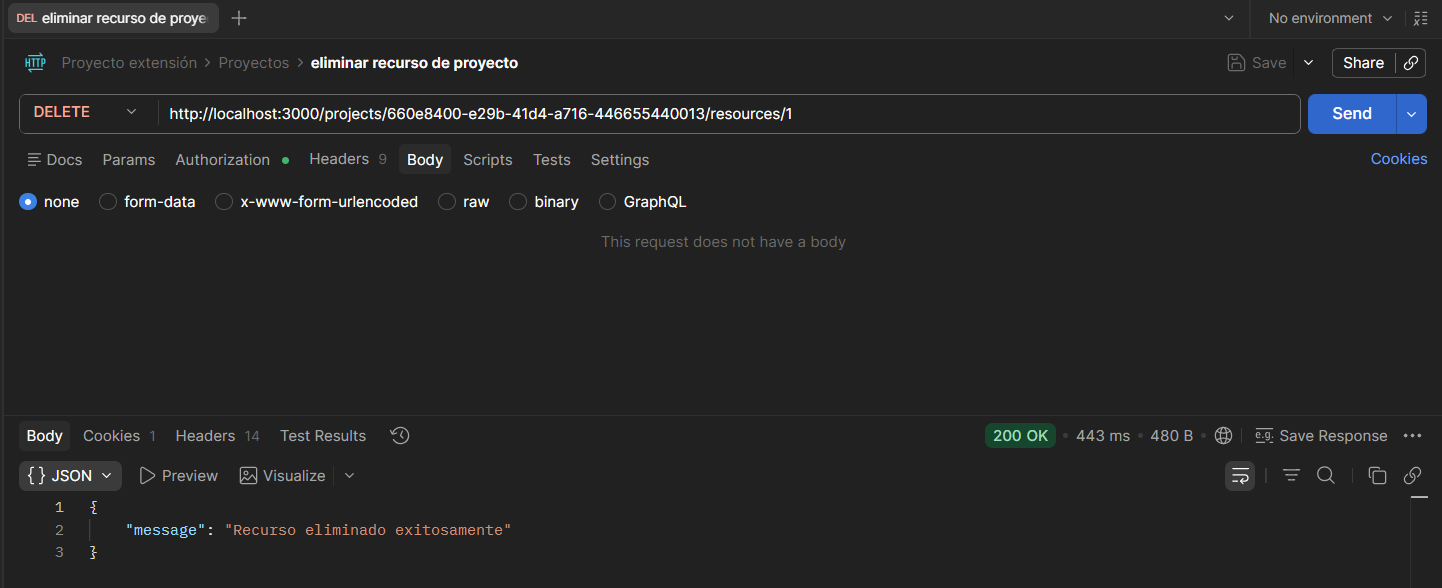
\includegraphics[width=0.88\textwidth]{assets/deleteResource.png}
                \caption{Eliminación de recurso - Prueba de éxito}
                \label{fig:deleteResource}
            \end{figure}
    \item \texttt{GET /ruta/inexistente}: Esta solicitud busca acceder a una ruta que no existe. El resultado esperado
        para esta prueba es un código de respuesta HTTP 404 con un mensaje de error que indica que la ruta no fue encontrada.
            \begin{figure}[H]
                \centering
                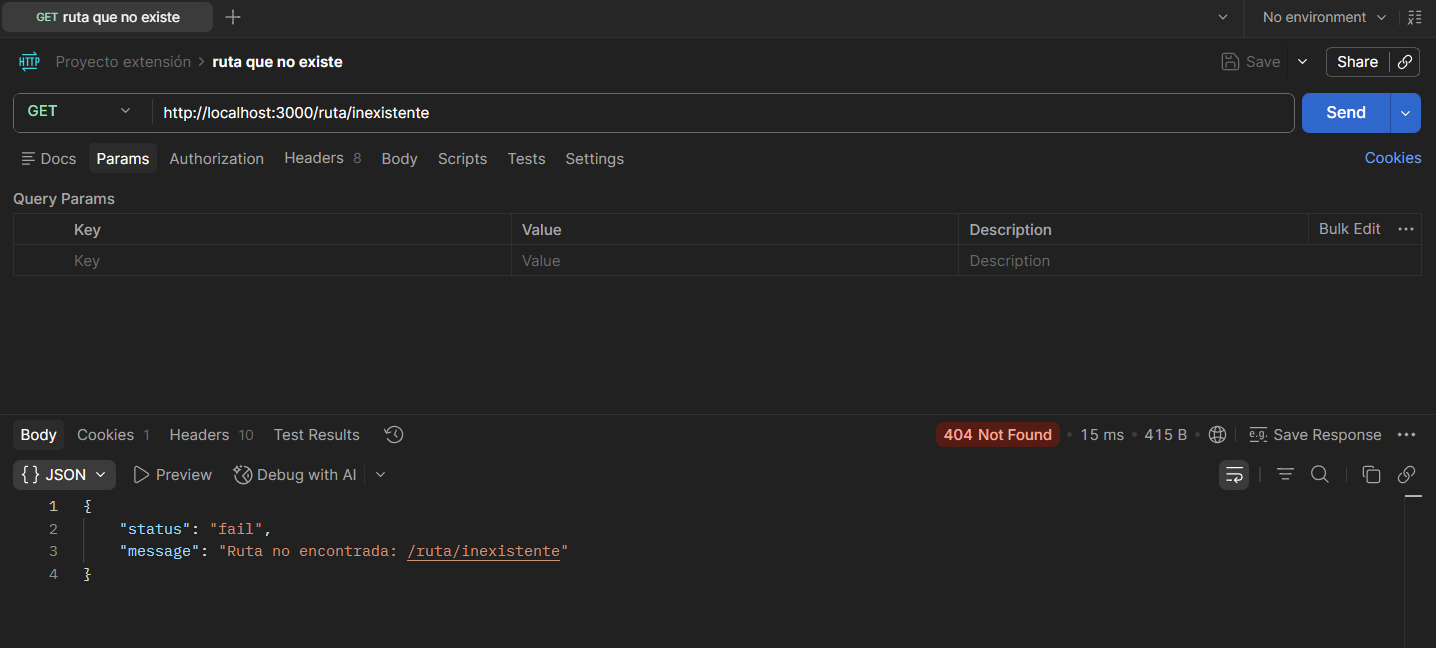
\includegraphics[width=0.88\textwidth]{assets/notFound.png}
                \caption{Ruta no encontrada - Prueba de error}
                \label{fig:notFound}
            \end{figure}
\end{itemize}

\subsection{Pruebas de estrés}
Con el fin de garantizar que la API puede manejar correctamente una cantidad considerable de solicitudes concurrentes, se realizaron pruebas
de estrés utilizando la herramienta \textit{Loader.io}.

Las pruebas de estrés se consideran exitosas si la API puede manejar la cantidad de solicitudes concurrentes sin presentar errores o caídas,
y si el tiempo de respuesta se mantiene dentro de un rango aceptable, lo cual se define como un tiempo de respuesta promedio inferior a 1s.

La lista completa de pruebas se encuentra en el Anexo \ref{anexo:pruebasestres}.
A continuación, se muestran los resultados obtenidos para las pruebas de estrés realizadas con diferentes niveles de concurrencia:
\begin{itemize}
    \item \texttt{GET /projects}: El tiempo de respuesta promedio fue de 18ms.
        \begin{figure}[H]
            \centering
            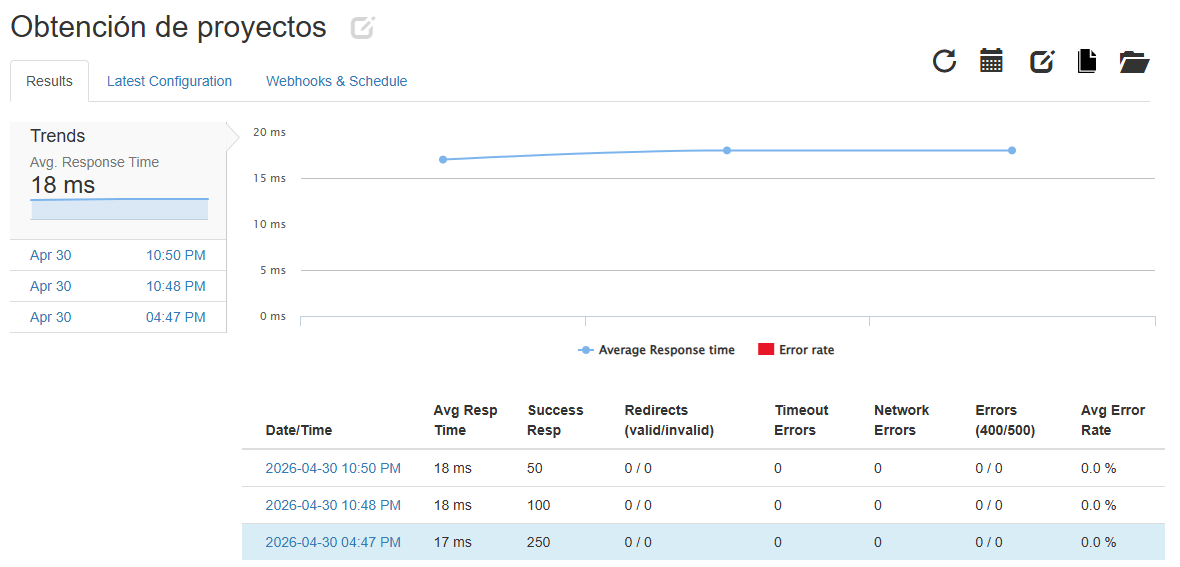
\includegraphics[width=0.88\textwidth]{assets/stressTestProjects.png}
            \caption{Prueba de estrés - GET /projects}
            \label{fig:stressTestProjects}
        \end{figure}
    \item \texttt{GET /projects/:projectId}: El tiempo de respuesta promedio fue de 21ms.
        \begin{figure}[H]
            \centering
            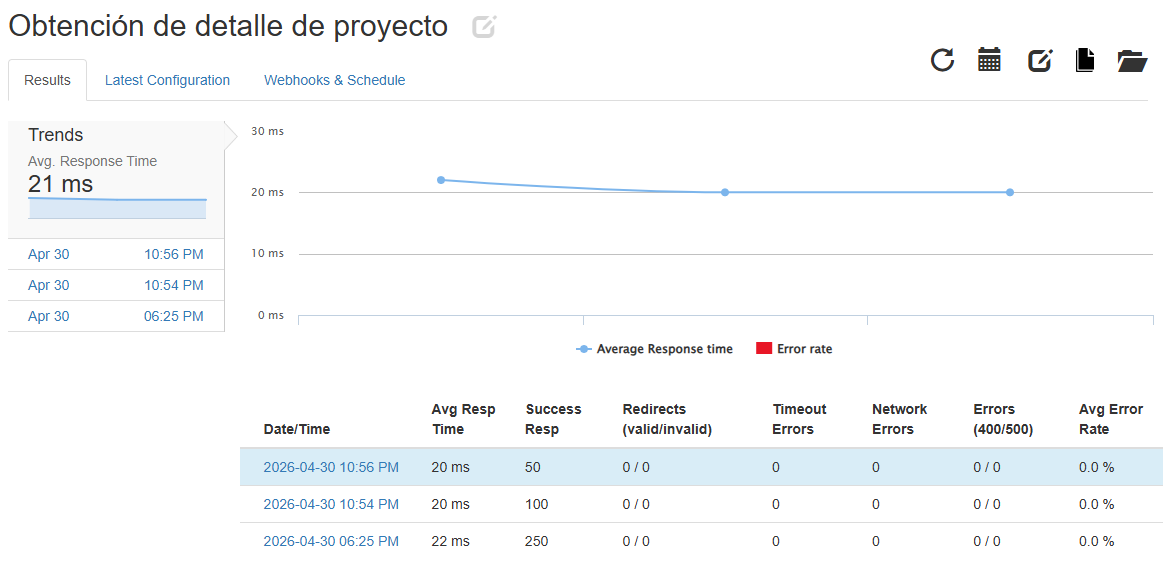
\includegraphics[width=0.88\textwidth]{assets/stressTestProjectById.png}
            \caption{Prueba de estrés - GET /projects/:projectId}
            \label{fig:stressTestProjectById}
        \end{figure}
    \item \texttt{GET /applications/completed}: El tiempo de respuesta promedio fue de 16ms.
        \begin{figure}[H]
            \centering
            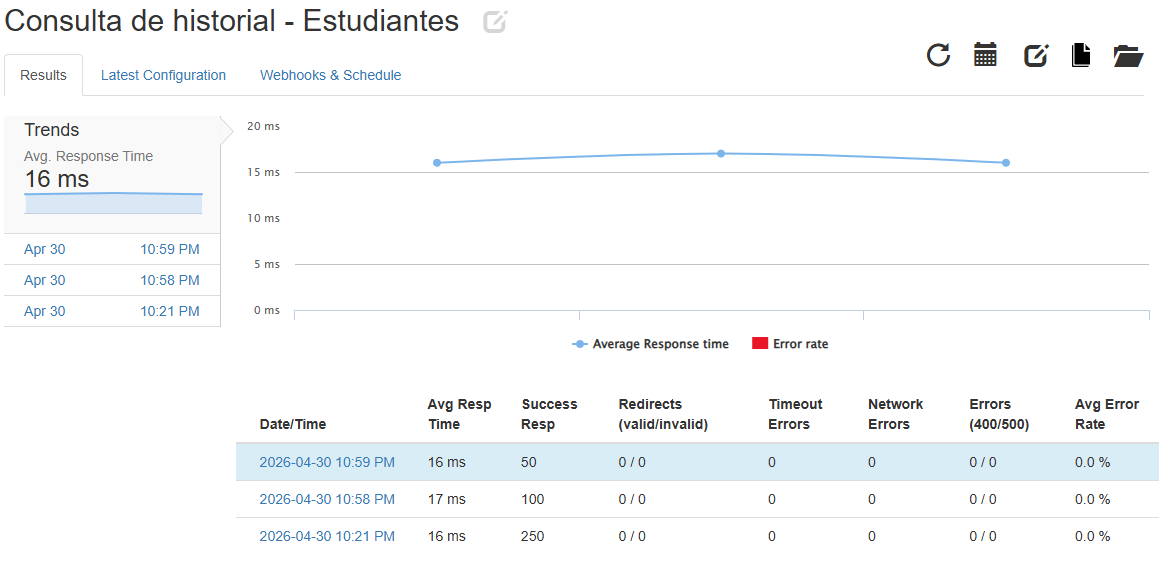
\includegraphics[width=0.88\textwidth]{assets/stressTestApplicationsCompleted.png}
            \caption{Prueba de estrés - GET /applications/completed}
            \label{fig:stressTestApplicationsCompleted}
        \end{figure}
    \item \texttt{GET /hours/total}: El tiempo de respuesta promedio fue de 16ms.
        \begin{figure}[H]
            \centering
            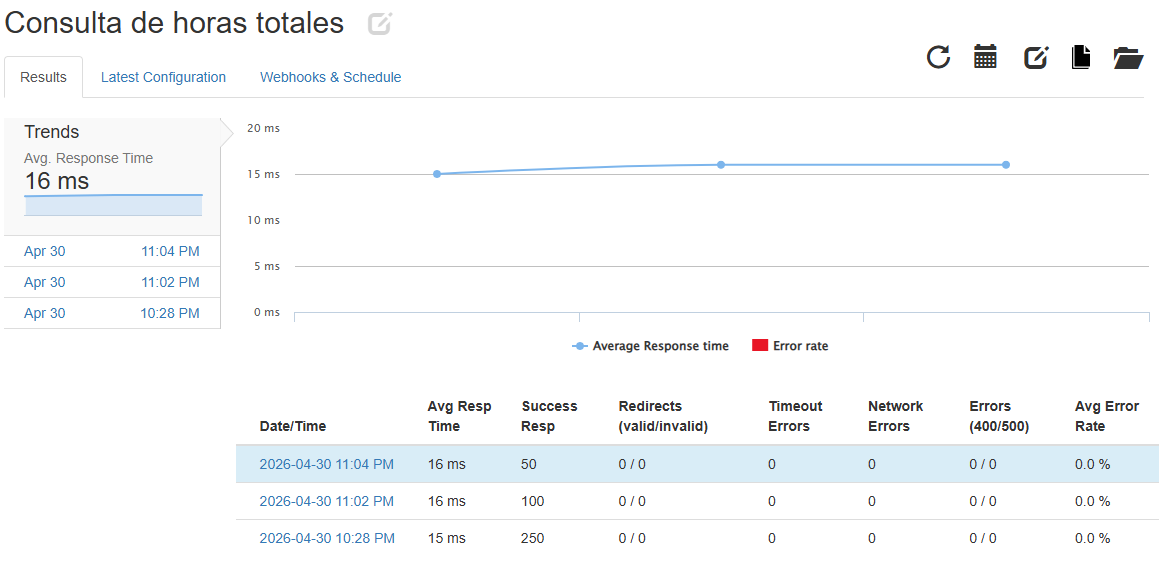
\includegraphics[width=0.88\textwidth]{assets/stressTestHoursTotal.png}
            \caption{Prueba de estrés - GET /hours/total}
            \label{fig:stressTestHoursTotal}
        \end{figure}
    \item \texttt{POST /auth/login}: El tiempo de respuesta promedio fue de 138ms.
        \begin{figure}[H]
            \centering
            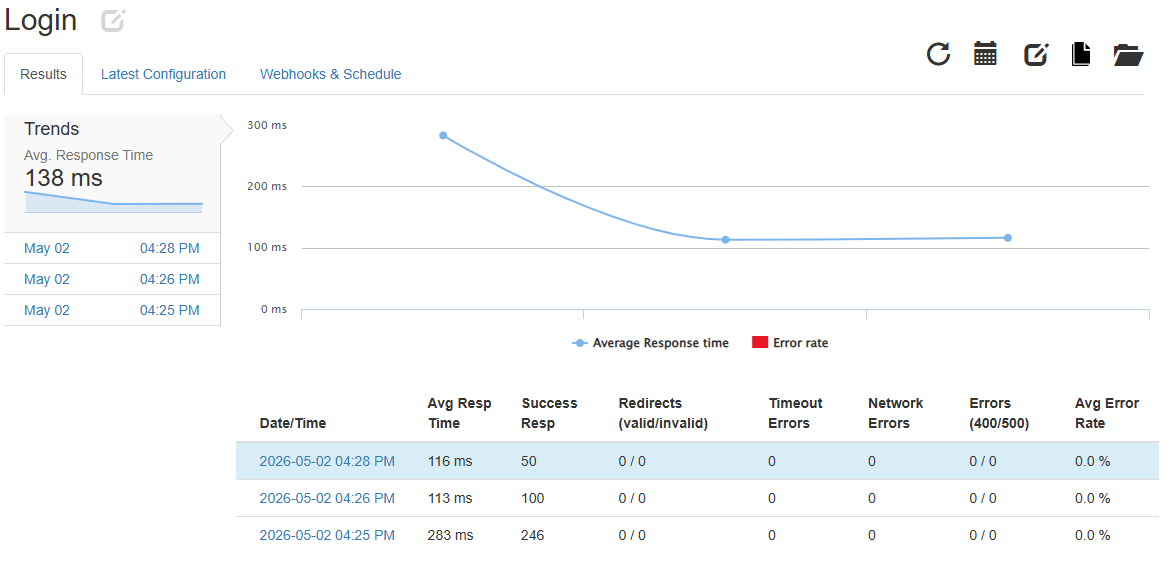
\includegraphics[width=0.88\textwidth]{assets/stressTestAuthLogin.png}
            \caption{Prueba de estrés - POST /auth/login}
            \label{fig:stressTestAuthLogin}
        \end{figure}
\end{itemize}

\section{Pruebas de usabilidad}
La implementación del \textit{Frontend} concluyó con pruebas de usabilidad realizadas por parte de usuarios finales, con el fin de garantizar
que la interfaz gráfica desarrollada a partir de los diseños previamente construidos y validados, permitan a los usuarios finales interactuar
con la plataforma para lograr realizar operaciones específicas para su rol, como lo son estudiantes, organizaciones externas y directores.
Las pruebas de usabilidad se consideran exitosas si los usuarios finales pueden realizar las operaciones esperadas sin dificultades significativas,
si la interfaz no presenta errores o comportamientos inesperados, y los resultados de la encuensta SUS se encuentra en un valor superior al promedio
de 68.

Las respuestas completas de las pruebas de usabilidad se encuentran en el Anexo \ref{anexo:resultadospruebasusabilidad}.

\subsection{Tareas}
Tal como se puede observar en la Figura \ref{fig:completedTasksGraph}, el 100\% de los participantes lograron completar las tareas asignadas.
\begin{figure}[H]
    \centering
    \begin{minipage}{0.44\textwidth}
        \centering
        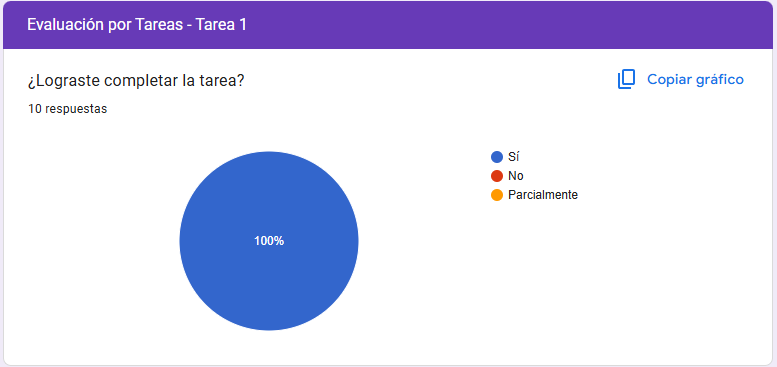
\includegraphics[width=\textwidth]{assets/completedTasksTarea1.png}
        \subcaption{Tarea 1}
    \end{minipage}
    \hfill
    \begin{minipage}{0.44\textwidth}
        \centering
        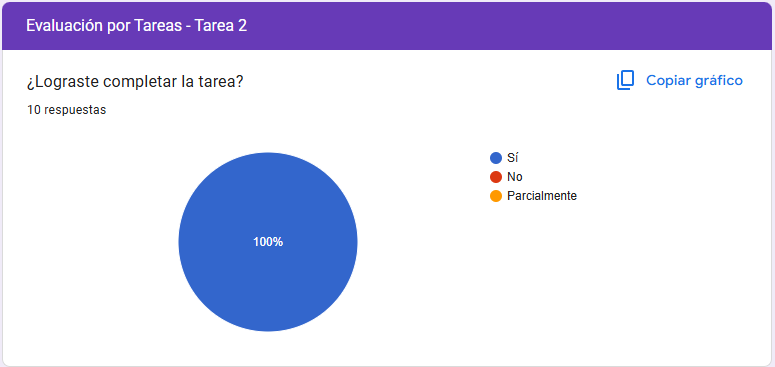
\includegraphics[width=\textwidth]{assets/completedTasksTarea2.png}
        \subcaption{Tarea 2}
    \end{minipage}
    \hfill
    \begin{minipage}{0.44\textwidth}
        \centering
        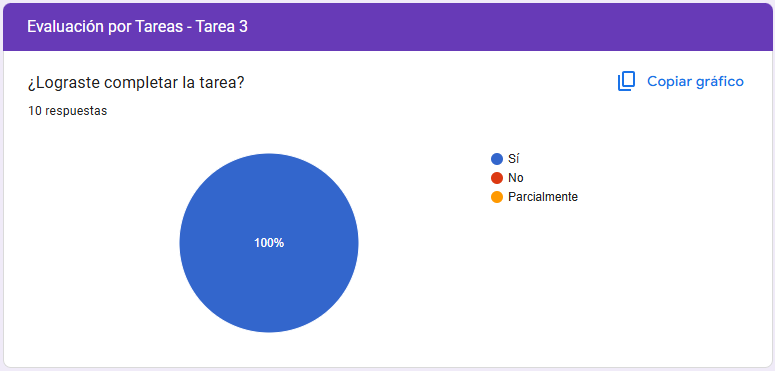
\includegraphics[width=\textwidth]{assets/completedTasksTarea3.png}
        \subcaption{Tarea 3}
    \end{minipage}
    \caption{Resultados de la Encuesta de Usabilidad - Sección de Evaluación de Tareas}
    \label{fig:completedTasksGraph}
\end{figure}

La dificultad percibida y el tiempo aproximado para completar cada tarea se muestra en la Figura \ref{fig:difficultyAndTimeGraph}.
\begin{figure}[H]
    \centering
    \begin{minipage}{0.44\textwidth}
        \centering
        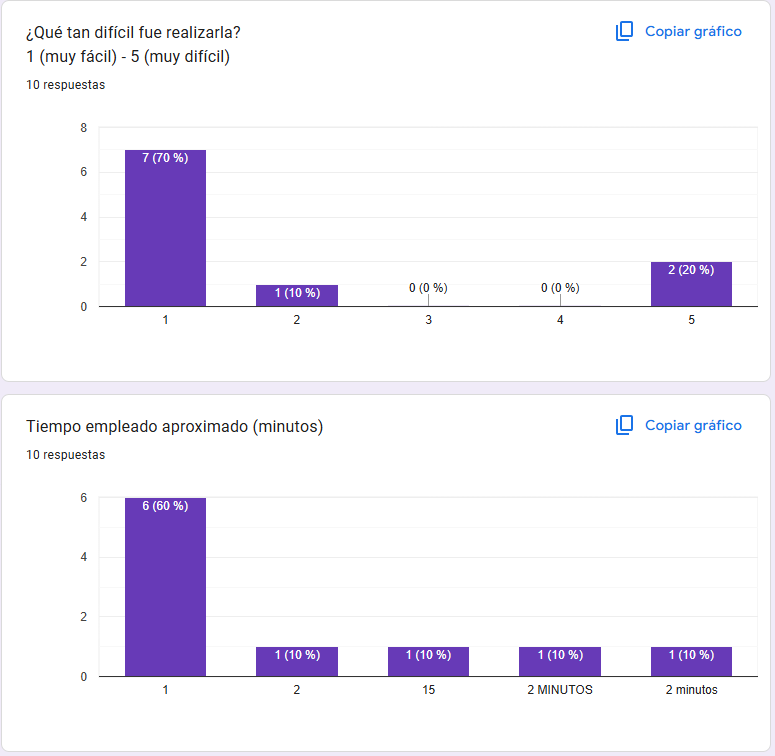
\includegraphics[width=\textwidth]{assets/difficultyAndTimeTarea1.png}
        \subcaption{Tarea 1}
    \end{minipage}
    \hfill
    \begin{minipage}{0.44\textwidth}
        \centering
        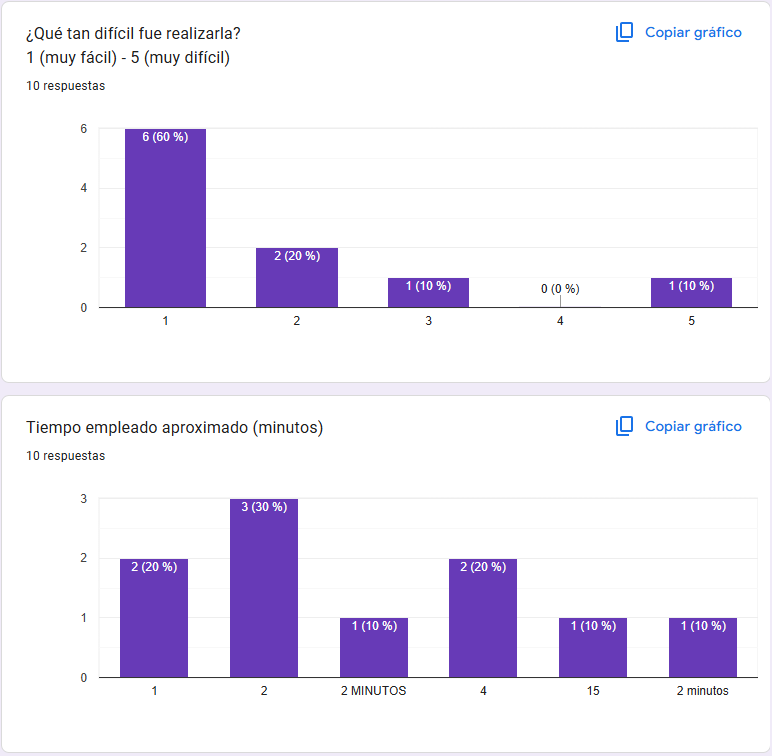
\includegraphics[width=\textwidth]{assets/difficultyAndTimeTarea2.png}
        \subcaption{Tarea 2}
    \end{minipage}
    \hfill
    \begin{minipage}{0.44\textwidth}
        \centering
        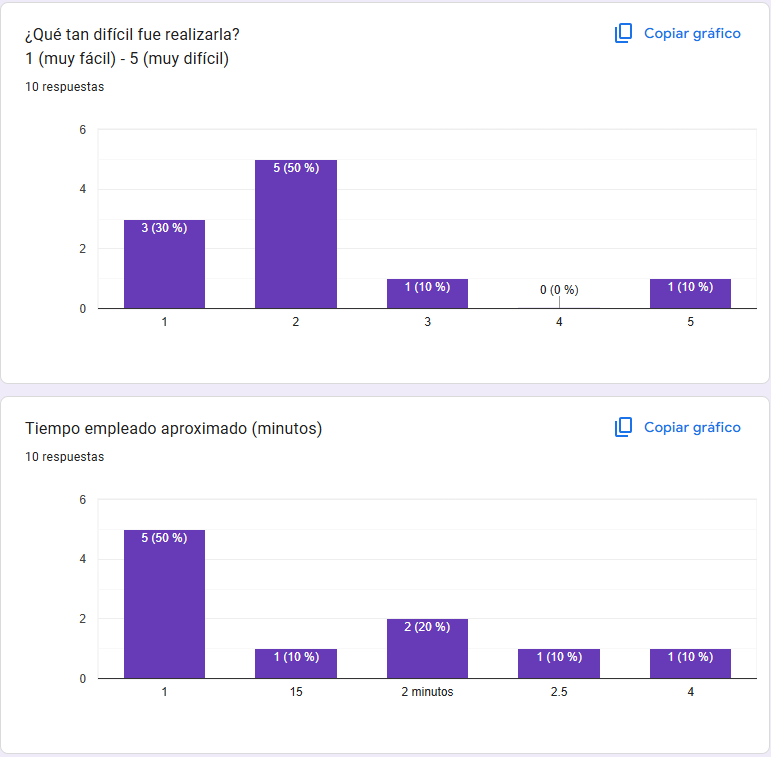
\includegraphics[width=\textwidth]{assets/difficultyAndTimeTarea3.png}
        \subcaption{Tarea 3}
    \end{minipage}
    \caption{Resultados de la Encuesta de Usabilidad - Sección de Evaluación de Tareas}
    \label{fig:difficultyAndTimeGraph}
\end{figure}

Algo por aclarar en estos resultados es que, algunos de los participantes respondieron de manera errónea la dificultad percibida, ya que aunque
en el cuestionario se indicó que 1 es muy fácil y 5 es muy difícil, algunos participantes respondieron con 5 para indicar que la tarea fue muy fácil,
lo cual se pudo corroborar con los tiempos aproximados para completar cada tarea, los cuales fueron menores a 2 minutos para los participantes
que respondieron con 5, lo cual indica que la tarea fue fácil de completar para ellos.

\subsubsection{Validación de cambios en la Base de Datos y Bucket S3}
En la Figura \ref{fig:usabilityTestDB} se muestra la validación de los cambios realizados en la Base de Datos durante una prueba de usabilidad,
en este caso, el participante era un estudiante que realizó actualización de su perfil, postulación a un proyecto de extensión y el registro
de horas de participación en un proyecto de extensión.
Se puede observar que los cambios realizados por el participante durante la prueba de usabilidad se reflejaron correctamente en la Base de Datos,
lo que indica que la plataforma web funciona correctamente en cuanto a la manipulación de datos y permite a los usuarios realizar las operaciones esperadas.

\begin{figure}[H]
    \centering
    \begin{minipage}{0.44\textwidth}
        \centering
        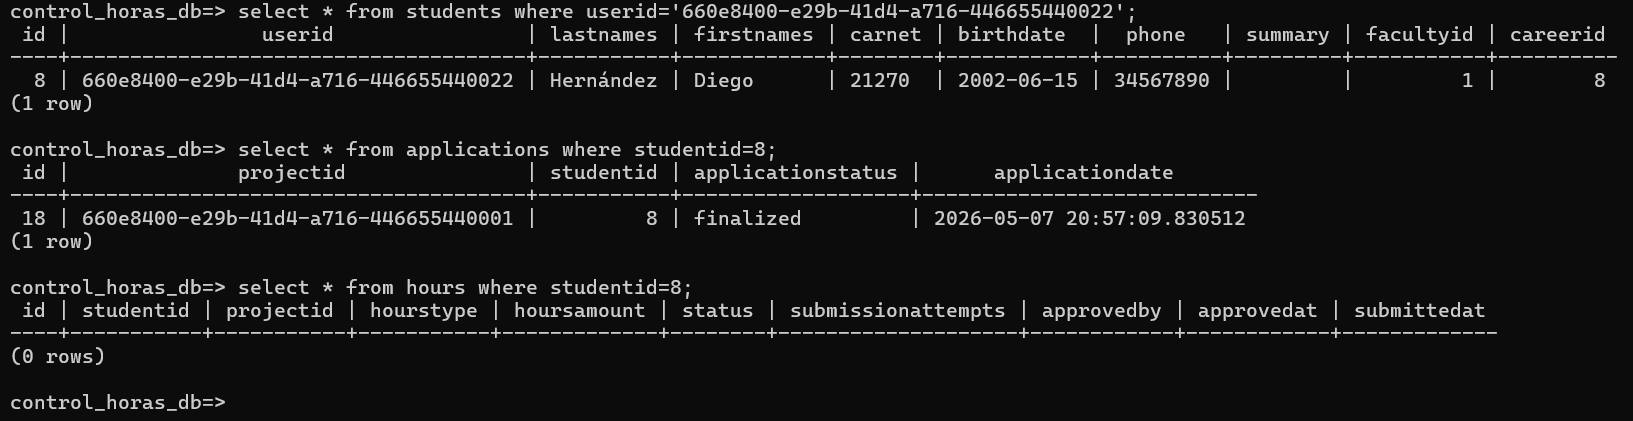
\includegraphics[width=\textwidth]{assets/usabilityTestDBbefore.png}
        \subcaption{Base de Datos antes de la prueba de usabilidad}
    \end{minipage}
    \hfill
    \begin{minipage}{0.44\textwidth}
        \centering
        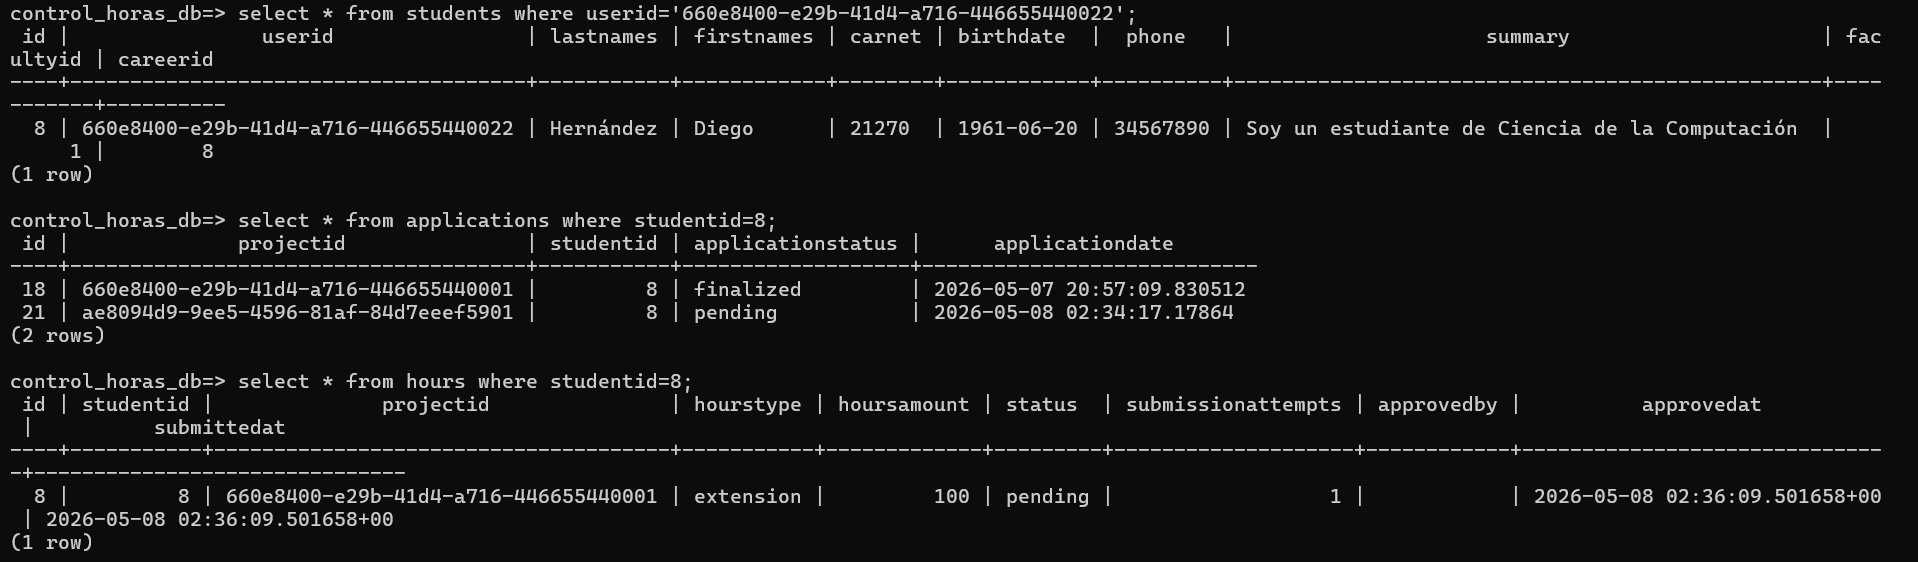
\includegraphics[width=\textwidth]{assets/usabilityTestDBafter.png}
        \subcaption{Base de Datos después de la prueba de usabilidad}
    \end{minipage}
    \caption{Validación de cambios en la Base de Datos - Prueba de Usabilidad}
    \label{fig:usabilityTestDB}
\end{figure}

En la Figura \ref{fig:usabilityTestBucketS3} se muestra la validación de los cambios realizados en el Bucket S3 durante una prueba de usabilidad,
en este caso, el participante era un estudiante que realizó la carga de un archivo de tipo evidencia de participación en un proyecto de extensión.
Se puede observar que el archivo se cargó correctamente en la carpeta esperada dentro del Bucket S3, y que los metadatos del archivo reflejan la
información correspondiente al proyecto de extensión al que se asoció el archivo y al usuario que realizó la carga, lo que indica que la plataforma
web funciona correctamente en cuanto a la manipulación de archivos y permite a los usuarios realizar las operaciones esperadas.
\begin{figure}[H]
    \centering
    \begin{minipage}{0.44\textwidth}
        \centering
        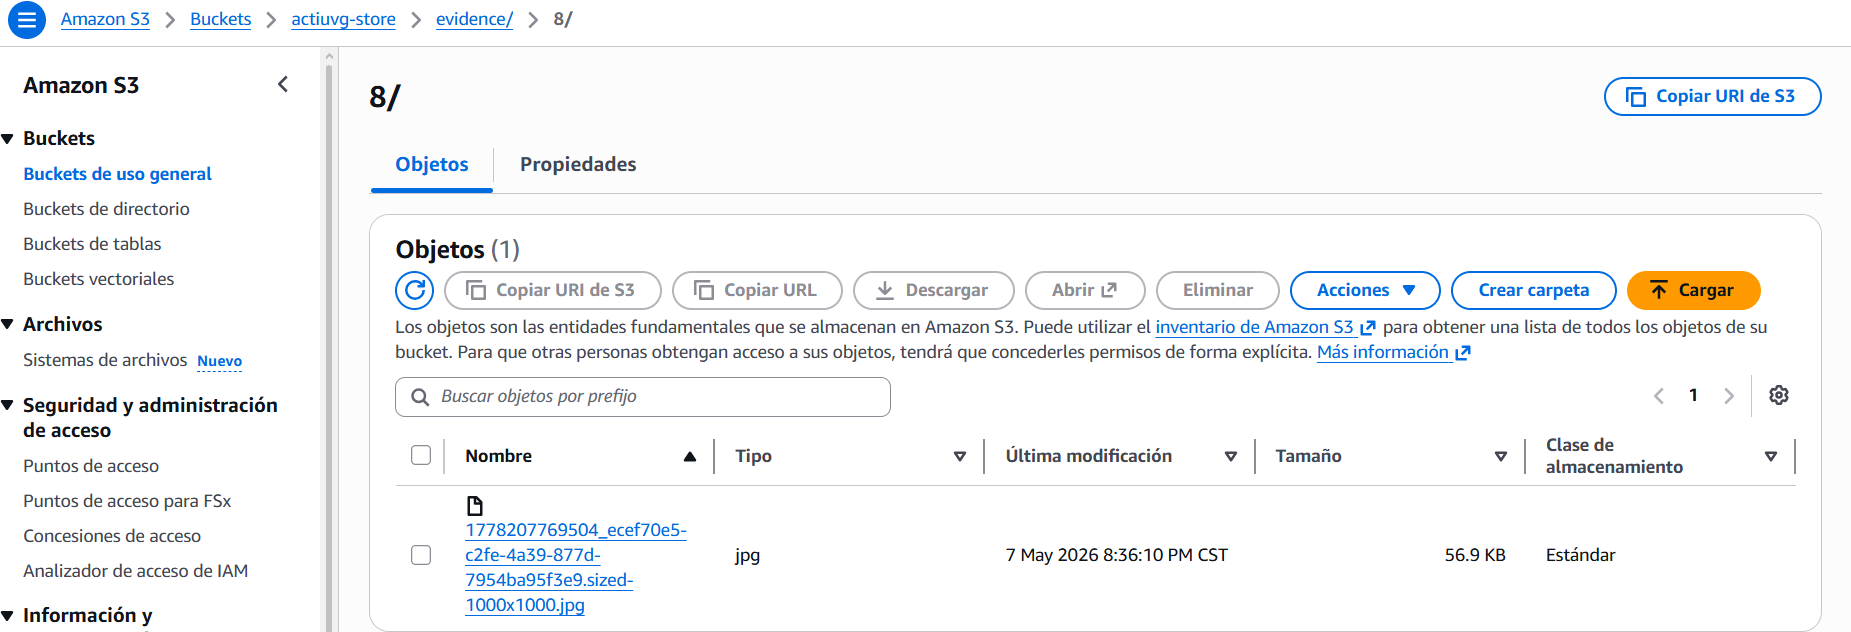
\includegraphics[width=0.88\textwidth]{assets/usabilityTestBucket.png}
        \subcaption{Archivo en el Bucket S3 de la prueba de usabilidad}
    \end{minipage}
    \hfill
    \begin{minipage}{0.44\textwidth}
        \centering
        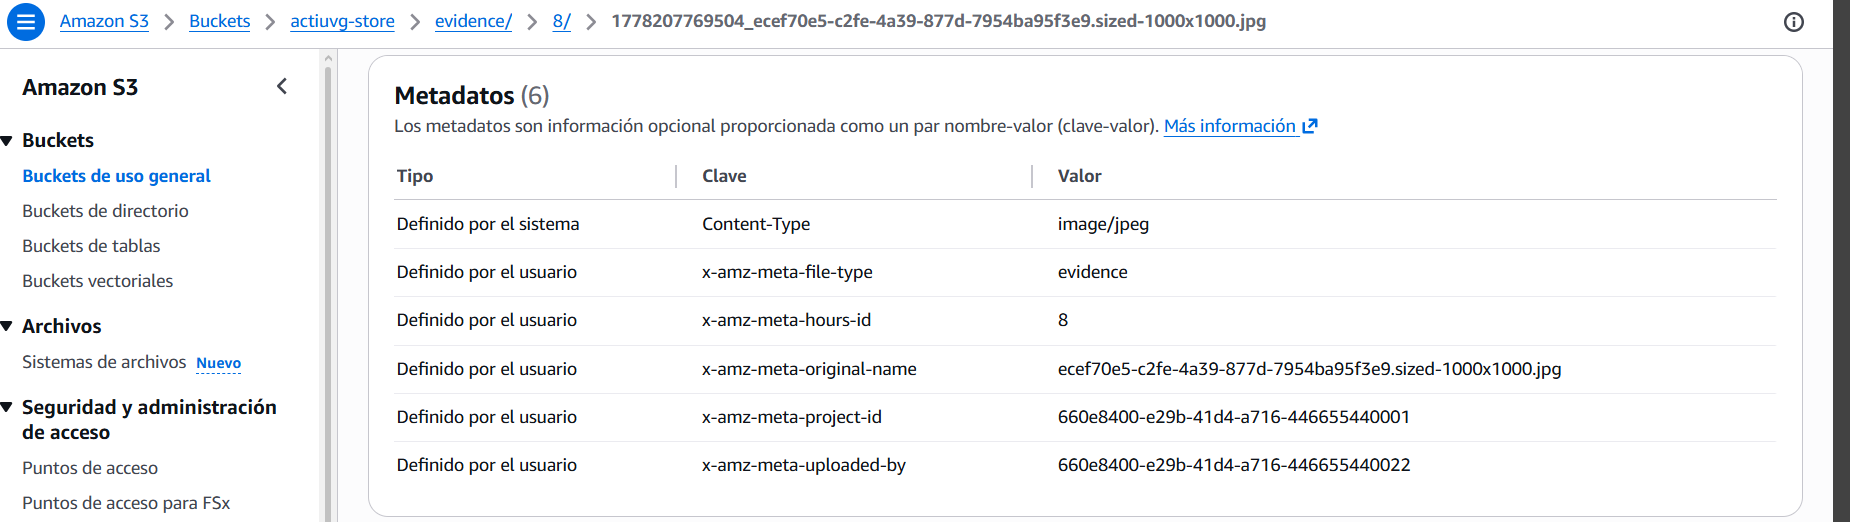
\includegraphics[width=0.88\textwidth]{assets/usabilityTestBucketMetadata.png}
        \subcaption{Metadatos del archivo en el Bucket S3 de la prueba de usabilidad}
    \end{minipage}
    \caption{Validación de cambios en el Bucket S3 - Prueba de Usabilidad}
    \label{fig:usabilityTestBucketS3}
\end{figure}

\subsection{SUS}
Las respuestas obtenidas para las preguntas SUS se muestran en la Figura \ref{fig:resultadosPreguntasSUS} y el cálculo del puntaje SUS a partir de
estas respuestas se muestra en la Figura \ref{fig:resultadoSUS}.

El puntaje promedio obtenido para las preguntas SUS fue de \textbf{80}, lo cual indica que la plataforma cuenta con una usabilidad excelente al estar por encima
del promedio de 68.

\section{Análisis de vulnerabilidades}
La plataforma web fue sometida a un análisis de vulnerabilidades utilizando la herramienta OWASP ZAP, esperando detectar posibles
vulnerabilidades de seguridad en la API y en el \textit{Frontend}. Se realizó un escaneo automatizado utilizando la funcionalidad
de \textit{Spider} y \textit{AJAX Spider}, seguido de un escaneo activo utilizando la funcionalidad de \textit{Active Scan}.
El resultado del análisis de vulnerabilidades no mostró ninguna alerta de seguridad crítica o alta, lo que indica que la plataforma
no presenta vulnerabilidades de seguridad significativas; sin embargo, sí mostró algunas alertas de seguridad de nivel medio y bajo,
las cuales fueron revisadas y mitigadas en la medida de lo posible, como la implementación o eliminación de encabezados HTTP.

\begin{figure}[H]
    \centering
    \begin{minipage}{0.44\textwidth}
        \centering
        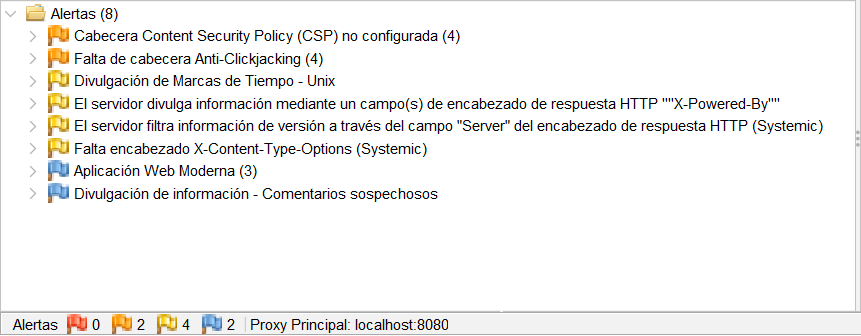
\includegraphics[width=\textwidth]{assets/zapInitial.png}
        \subcaption{Análisis inicial de vulnerabilidades - OWASP ZAP}
    \end{minipage}
    \hfill
    \begin{minipage}{0.44\textwidth}
        \centering
        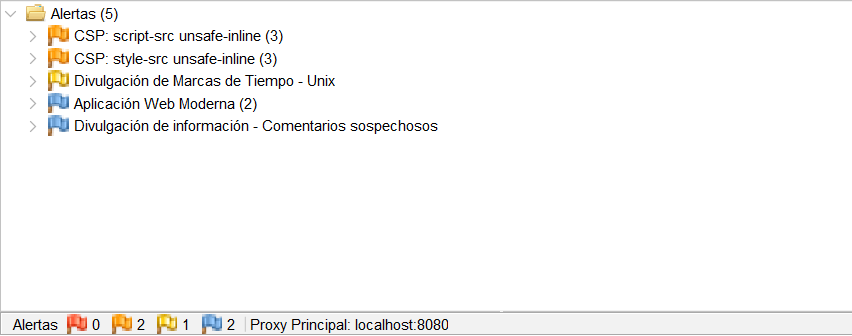
\includegraphics[width=\textwidth]{assets/zapFinal.png}
        \subcaption{Análisis final de vulnerabilidades - OWASP ZAP}
    \end{minipage}
    \caption{Análisis de vulnerabilidades - OWASP ZAP}
    \label{fig:vulnerabilities}
\end{figure}

